\documentclass[12pt]{article}

\usepackage[T1]{fontenc}
\usepackage[french]{babel}
\usepackage{geometry}
\usepackage{graphicx}
\usepackage{float}  % Pour le contrôle du placement des figures

\geometry{a4paper, margin=1in}

% Title settings
\title{
  \vspace{2cm}
  \textbf{\huge Projet d'optimisation continue}\\ 
  \textbf{\Large Estimation robuste du centre d’une pièce circulaire}
  \vspace{2cm}
}
\author{\textbf{EL GOTE Ismail}}
\date{\today}

\begin{document}
\maketitle
\newpage

\section*{Introduction}

Ce projet porte sur l'estimation robuste du centre d'une pièce mécanique circulaire à partir de mesures effectuées sur son contour. Ces mesures, représentées par des points \((x_i, y_i)\), sont entachées d'erreurs, certaines étant particulièrement aberrantes (outliers). 

L'objectif est de déterminer les coordonnées du centre du cercle \((c_x, c_y)\) en minimisant l'écart entre les distances des points mesurés et le rayon connu \(R\). Ce problème sera abordé à l'aide de méthodes d'optimisation continue, notamment les moindres carrés et des algorithmes comme la descente de gradient ou les méthodes quasi-Newton.

Ce travail permet d'appliquer des concepts théoriques d'optimisation à un problème concret tout en étudiant la robustesse des solutions proposées face à des données bruitées.

\section{Estimation au sens des moindres distances carrées (total least squares)}

\subsection{Question 1}

La fonction de coût est représentée dans l'espace des paramètres \((c_x, c_y)\) pour deux intervalles distincts. Le premier intervalle, \([-1, 1] \times [-1, 2]\), est illustré dans la figure 1, tandis que le second, \([-1, 4] \times [-1, 4]\), est présenté dans la figure 2.

\begin{figure}[H]
    \centering
    \begin{minipage}[b]{0.45\textwidth}
        \centering
        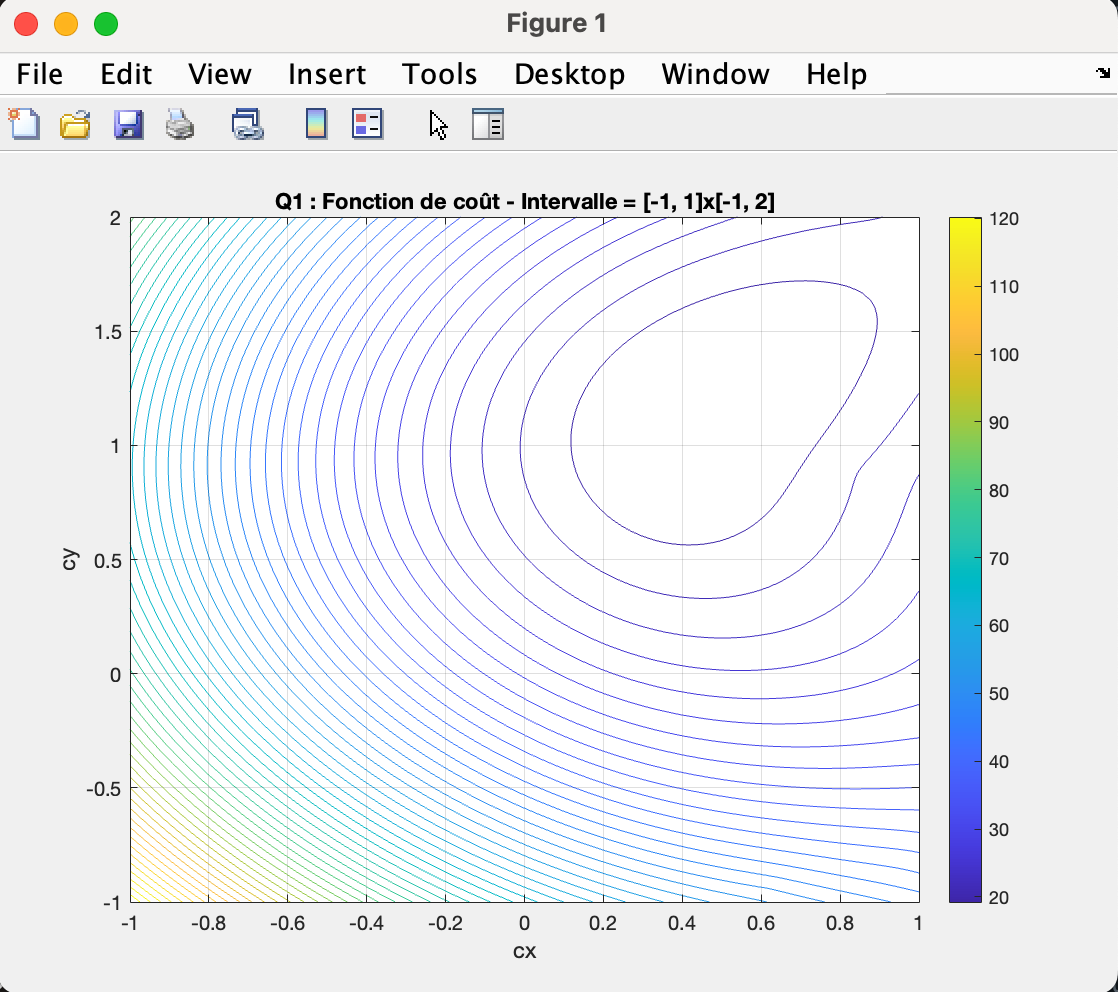
\includegraphics[width=\textwidth]{Q1.2.png} 
        \caption{Représentation de la fonction de coût pour l'intervalle \([-1, 1] \times [-1, 2]\)}
    \end{minipage}
    \hfill
    \begin{minipage}[b]{0.45\textwidth}
        \centering
        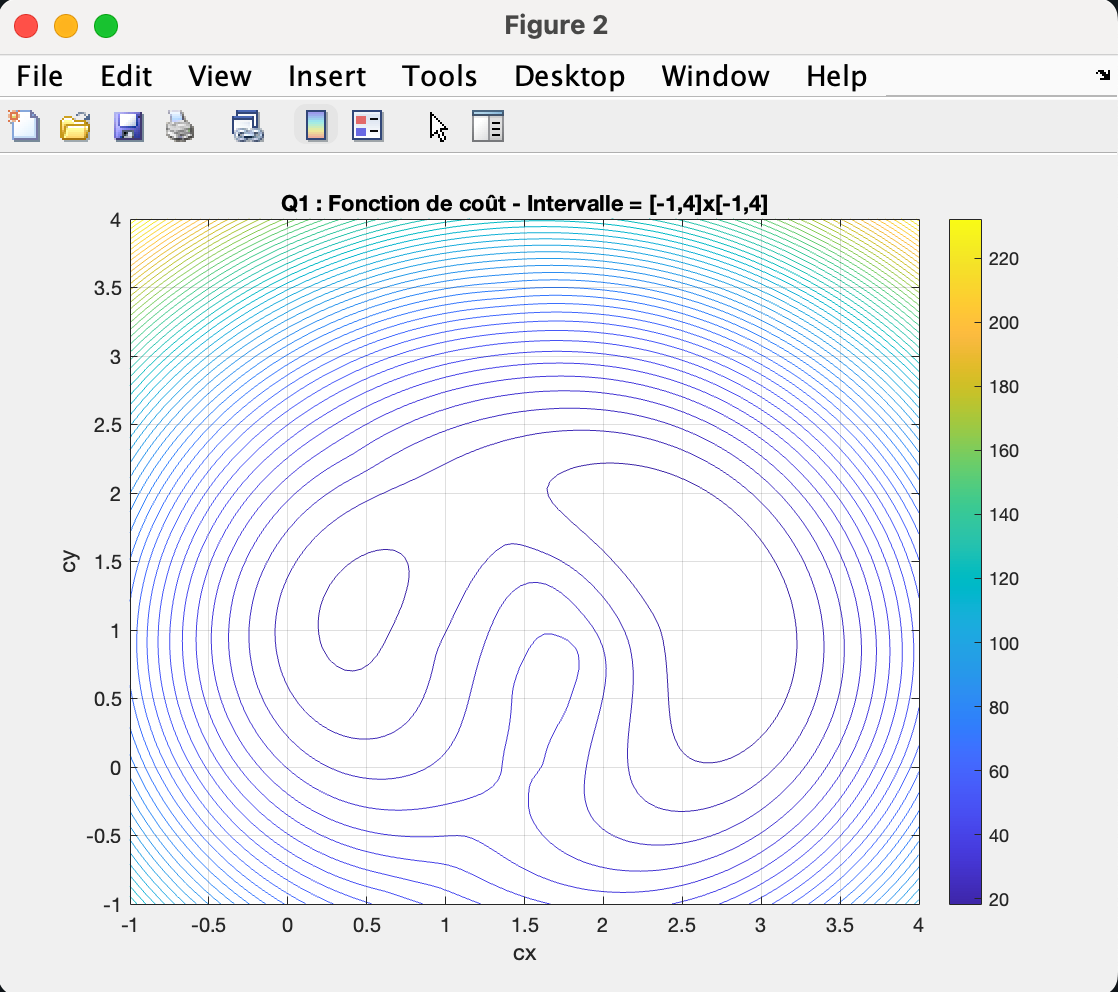
\includegraphics[width=\textwidth]{Q1.1.png}
        \caption{Représentation de la fonction de coût pour l'intervalle \([-1, 4] \times [-1, 4]\)}
    \end{minipage}
\end{figure}
En étendant l’intervalle d’analyse à \([-1, 4] \times [-1, 4]\), un second puits devient apparent, un phénomène qui n’était pas observable dans la représentation obtenue avec l’intervalle \(\emptyset\). Toutefois, dans l’optique d’identifier un minimum global, et non un minimum local, il semble plus judicieux de privilégier un intervalle plus vaste.
\subsection{Question 2}

\begin{figure}[H]
    \centering
    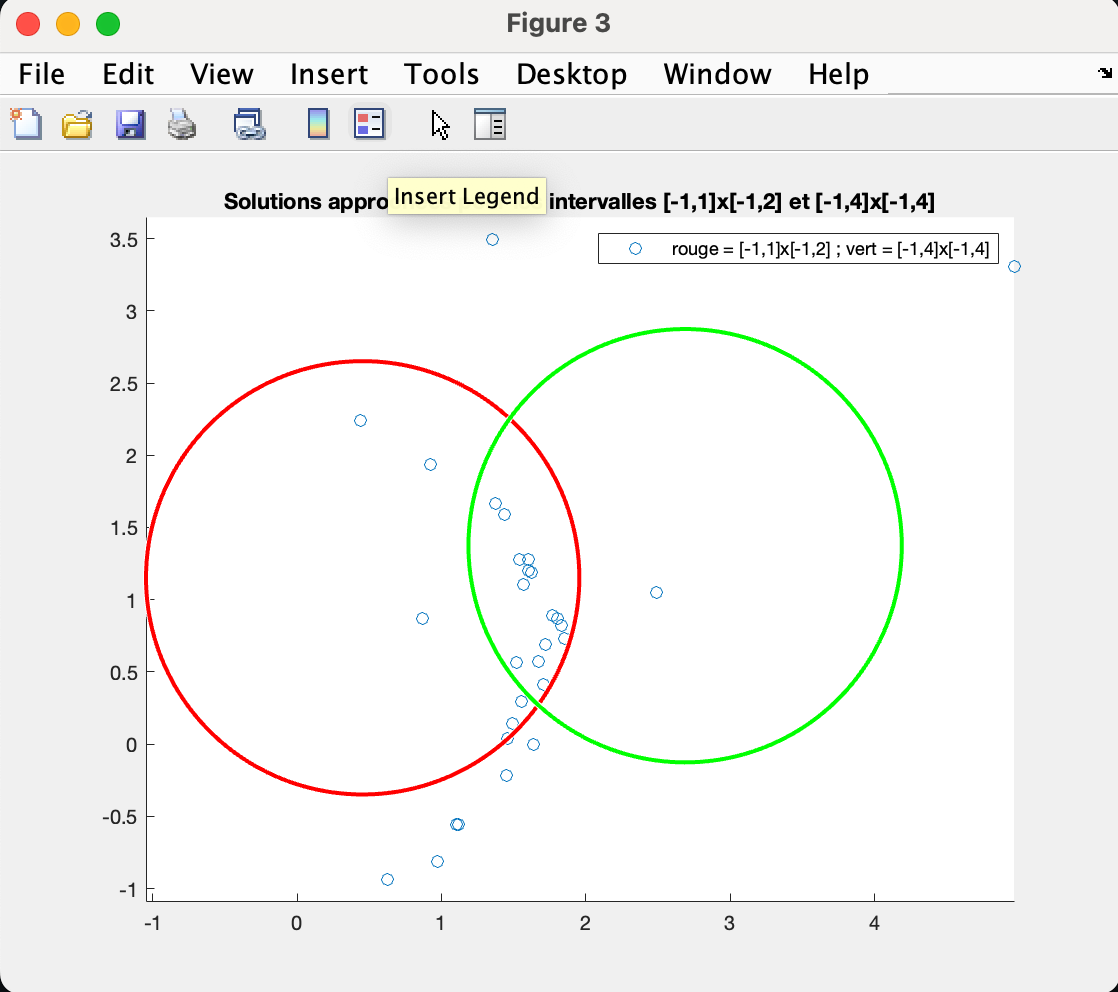
\includegraphics[width=0.8\textwidth]{Q2.png} 
    \caption{Solutions approchées pour les intervalles \([-1, 1] \times [-1, 2]\) et \([-1, 4] \times [-1, 4]\)}
\end{figure}
Pour obtenir les valeurs de \( c_x \) et \( c_y \) à l'aide de cette technique d’échantillonnage, il est indispensable d’évaluer la fonction un nombre total de \( n \times m \) fois, où \( n \) et \( m \) désignent les dimensions de la matrice, afin de tester chaque élément. Avec une précision de \( 10^{-4} \), pour un intervalle de type \([-1, 1] \times [-1, 2]\), il sera nécessaire de réaliser \( n \times m \) évaluations.

Dans le cas où l’intervalle est étendu à \([-1, 4] \times [-1, 4]\), le nombre d’évaluations à effectuer sera également de \( n \times m \).

Si l’on devait aussi calculer \( R \), il serait nécessaire d’ajouter une boucle \texttt{for} supplémentaire à chaque itération, ce qui multiplierait le temps de calcul par un facteur de \( 10^4 \). Bien que cette méthode soit d'une grande précision, le temps de calcul deviendrait excessivement long pour un projet de cette envergure.

\subsection{Question 3}

Voici l'expression du gradient de la fonction de coût :
\begin{figure}[H]
    \centering
    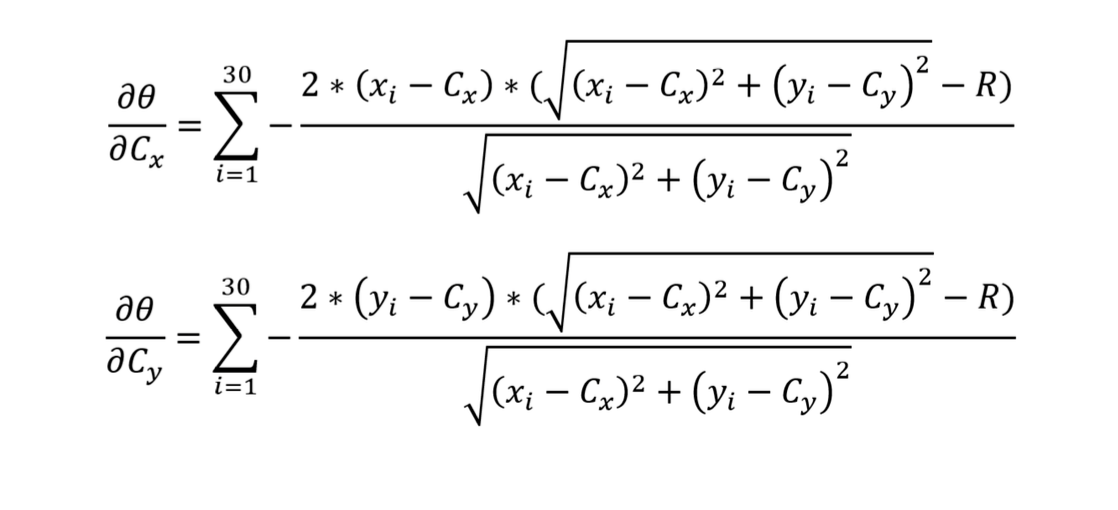
\includegraphics[width=0.8\textwidth]{Q3.png} 
    \caption{Expression du gradient de la fonction de coût}
\end{figure}

\subsection{Question 4}
En prenant le point \(0,0\), on obtient des valeurs extrêmement proches les unes par rapport aux autres
\begin{figure}[H]
    \centering
    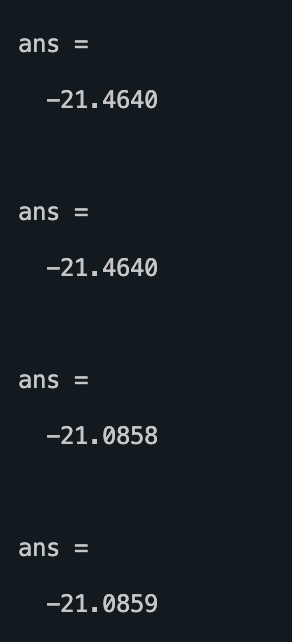
\includegraphics[width=0.3\textwidth]{Q4.png} 
    \caption{Valeurs obtenues pour le point \(0,0\)}
\end{figure}

\subsection{Question 5}

\begin{figure}[H]
    \centering
    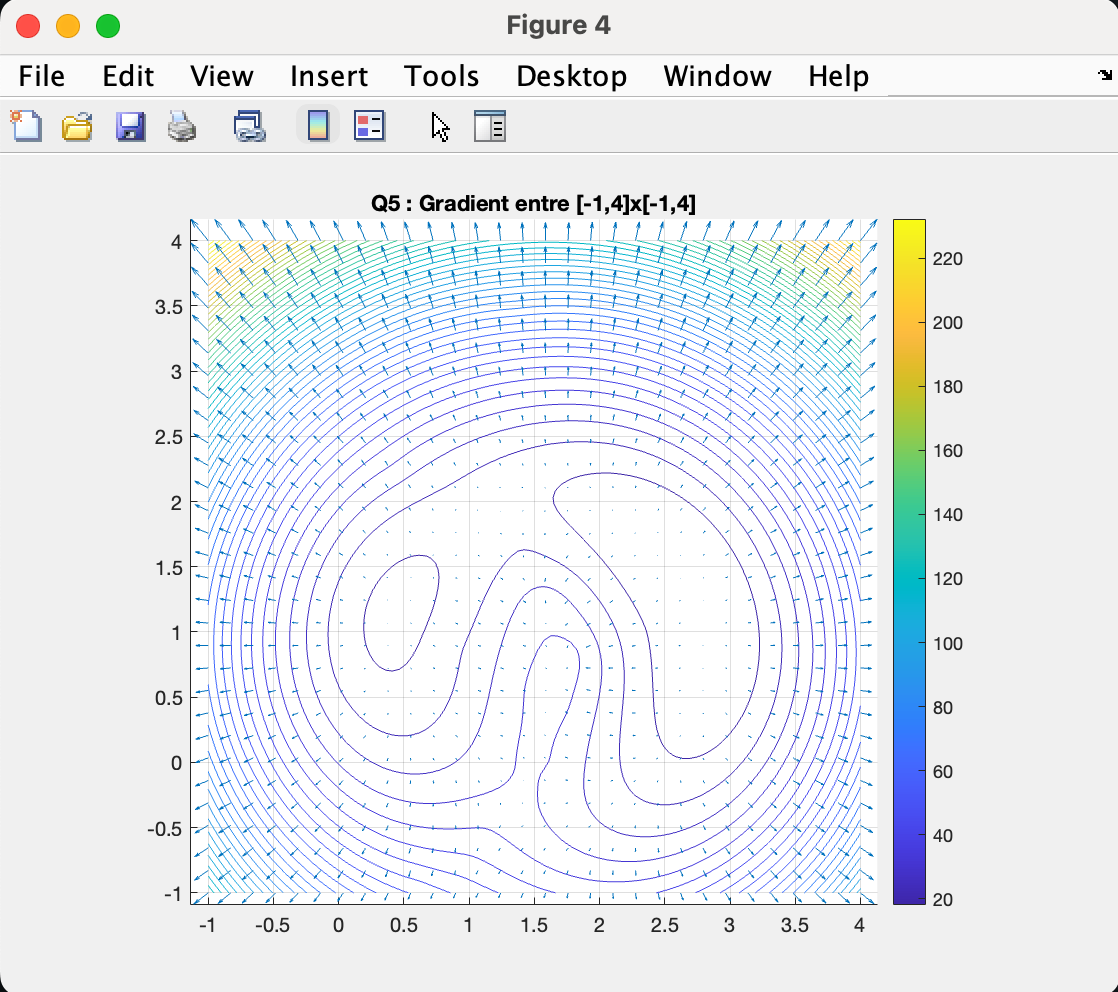
\includegraphics[width=0.8\textwidth]{Q5.png} 
    \caption{Q5 : Gradient entre [-1,4]x[-1,4]}
\end{figure}
Il ressort clairement que les vecteurs associés au gradient se trouvent parfaitement perpendiculaires aux courbes de niveau, ce qui atteste de l’exactitude de l’implémentation de la fonction gradient.

\subsection{Question 6}
\begin{figure}[H]
    \centering
    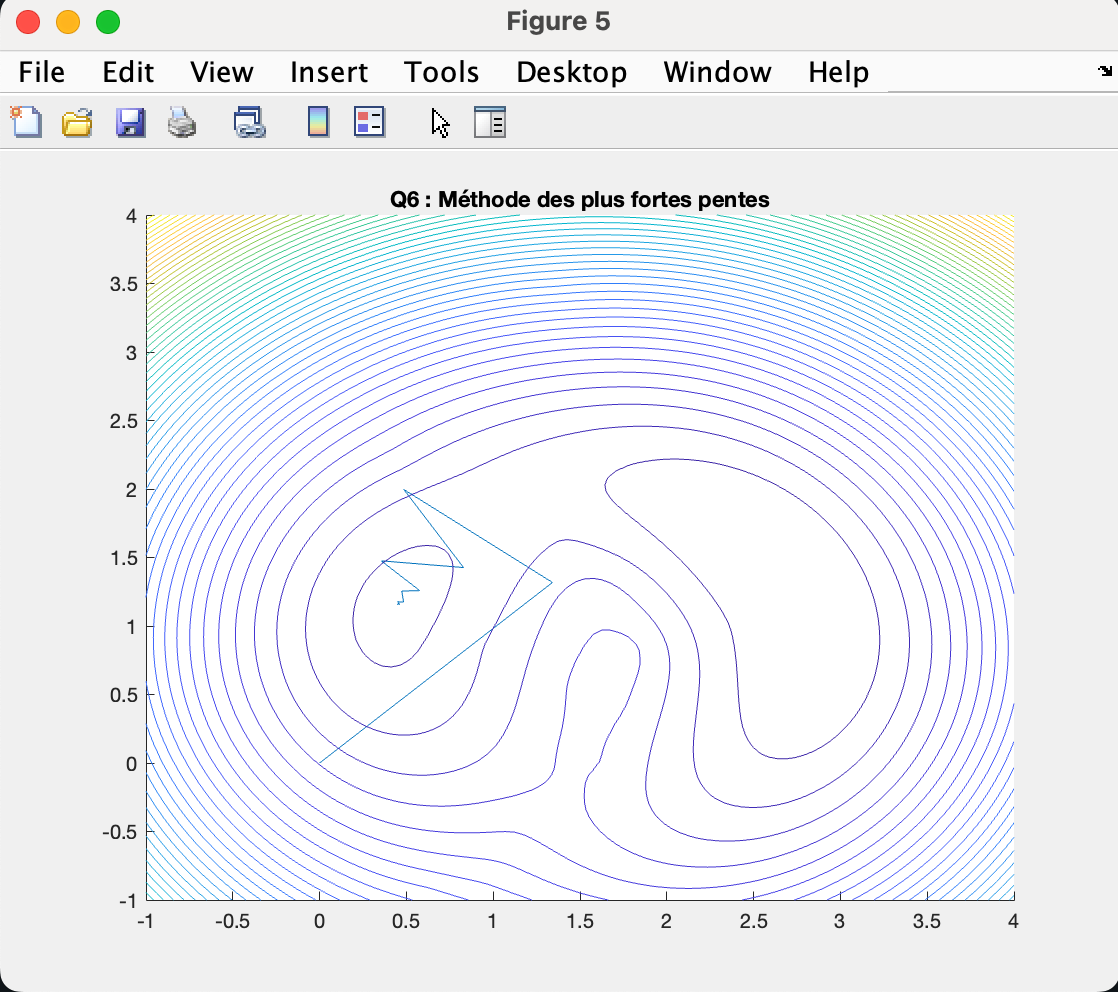
\includegraphics[width=0.8\textwidth]{Q6.1.png} 
    \caption{Q6 : Méthode des plus fortes pentes}
\end{figure}
\begin{figure}[H]
    \centering
    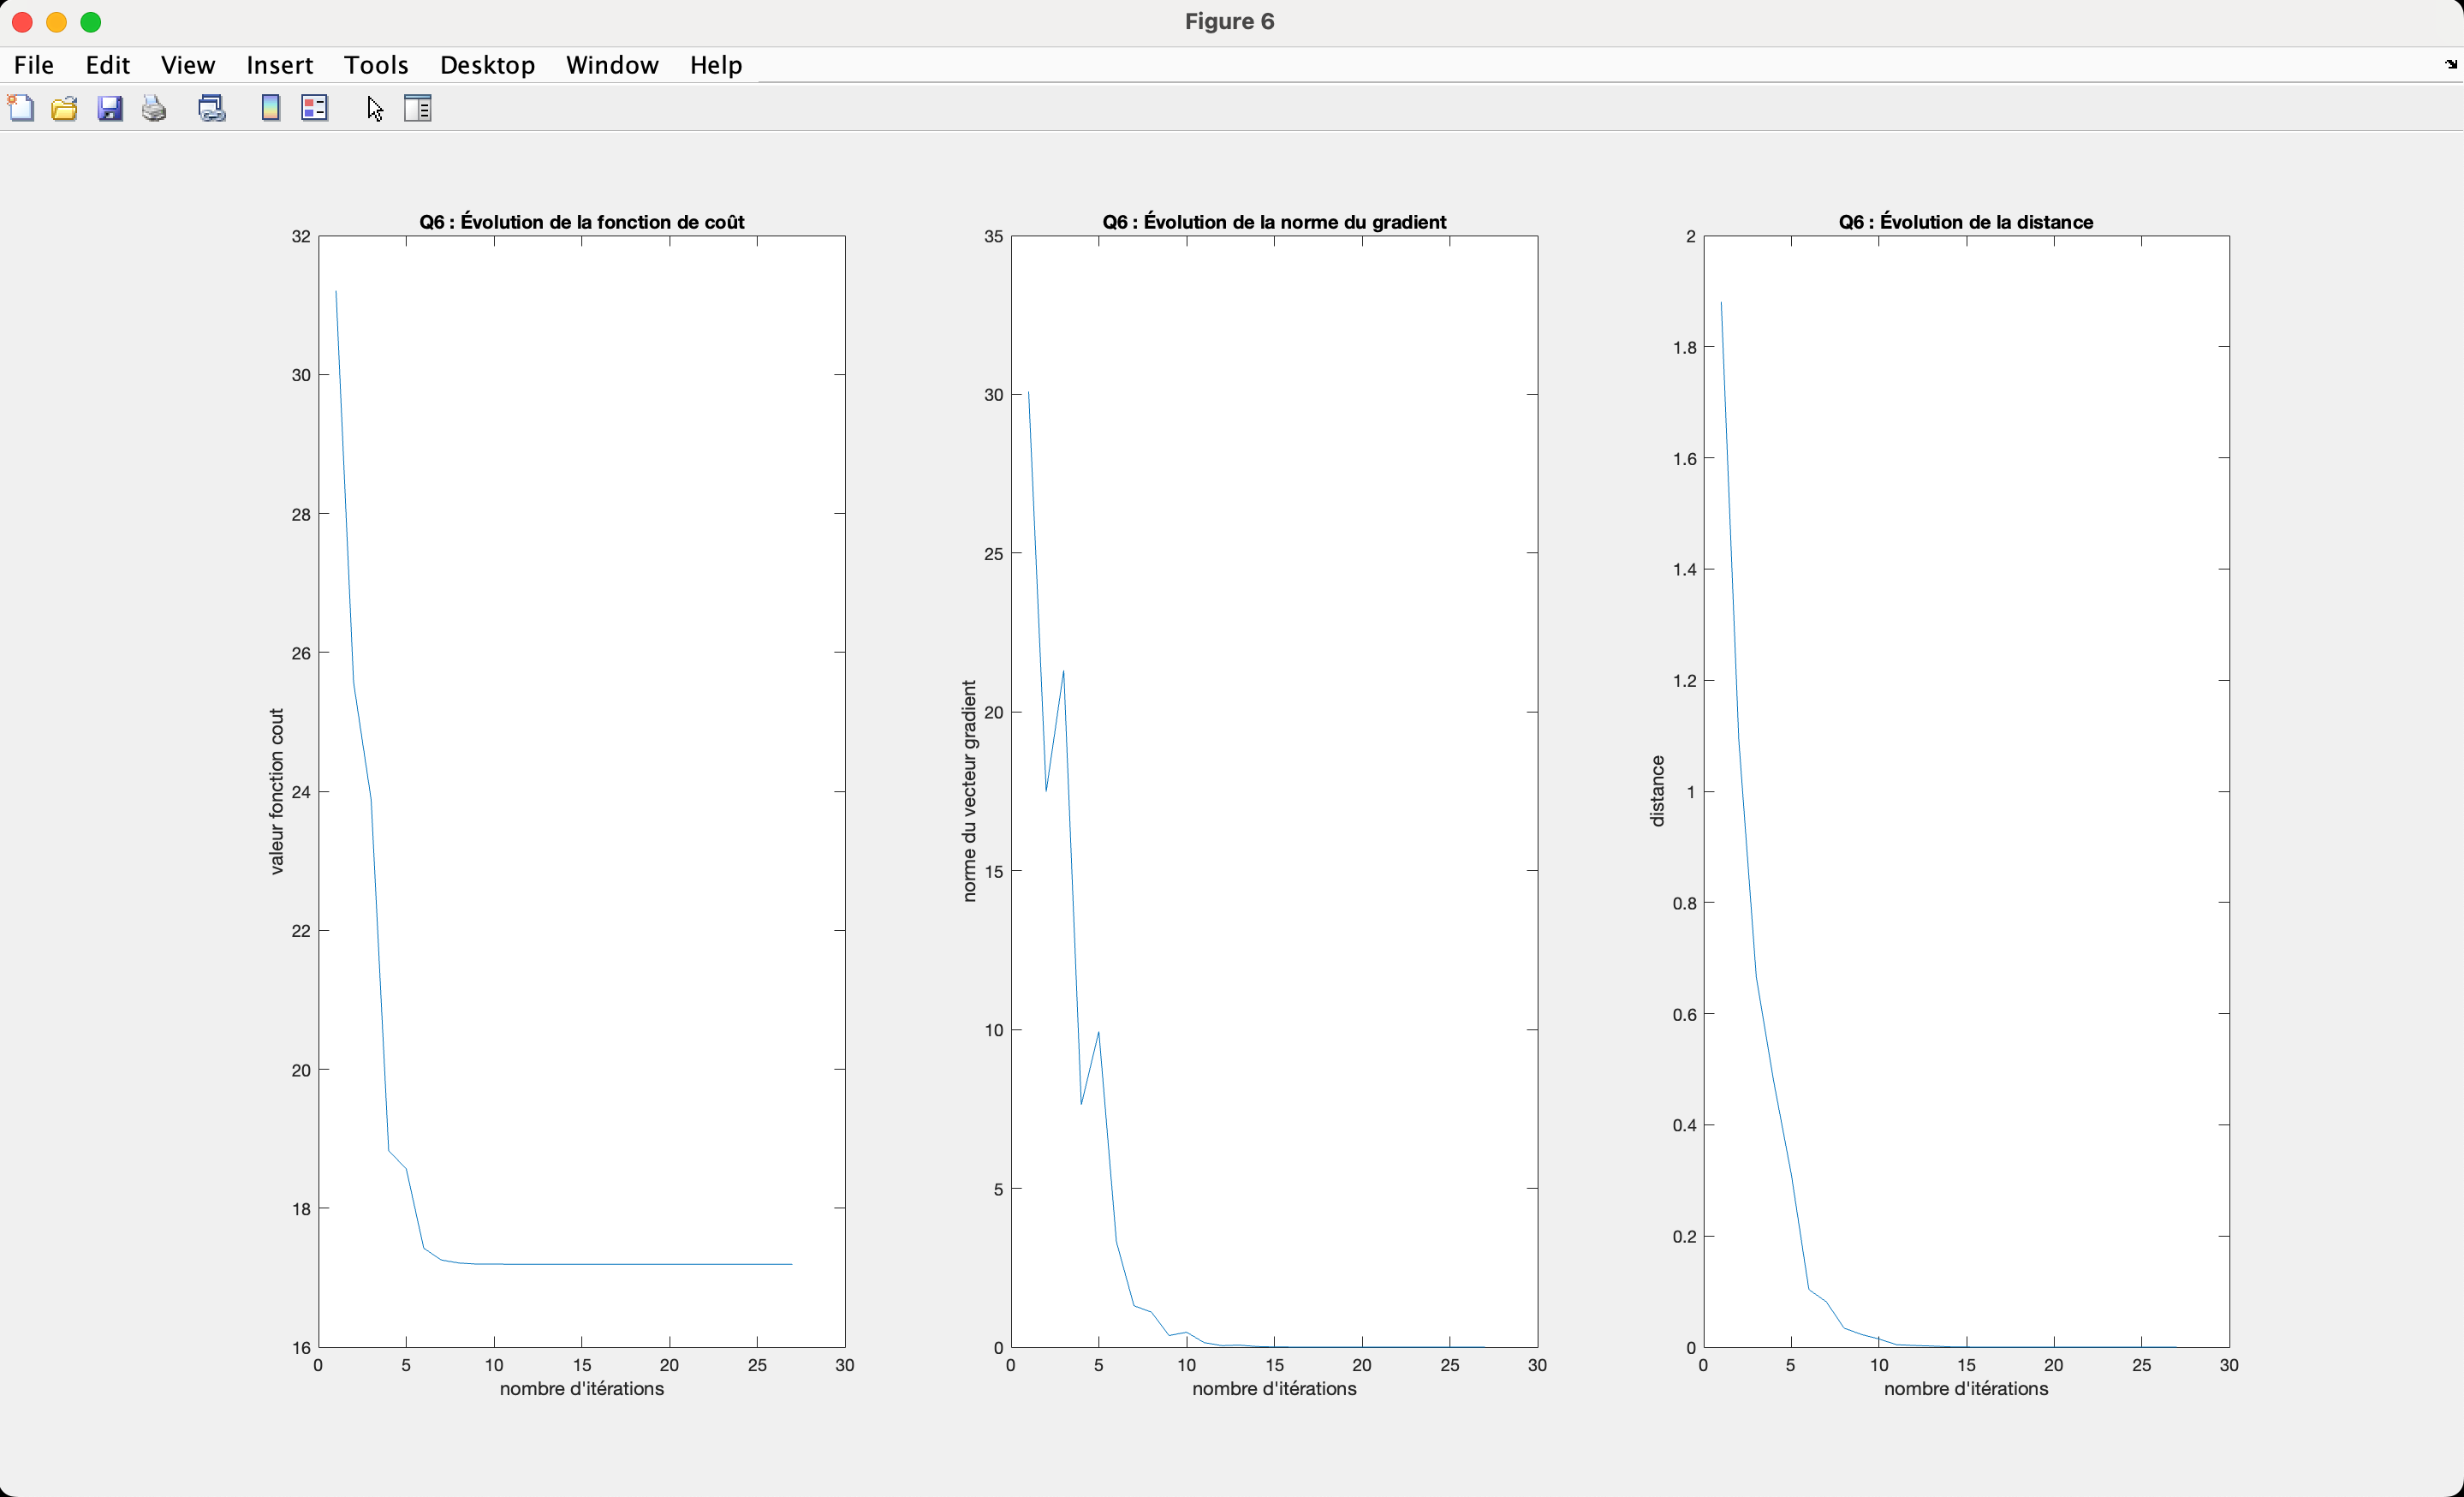
\includegraphics[width=0.8\textwidth]{Q6.2.png} 
    \caption{Q6 : Evolution des différentes caractéristiques demandées}
\end{figure}
Il est observé, comme le montre la figure 6, qu’en partant du point initial (0,0), on parvient au point central du puits, lequel représente un minimum. En effet, d’une part, l’évolution de la norme du gradient (figure 7) converge vers zéro à mesure que l’on se rapproche de ce minimum. D’autre part, au fur et à mesure des itérations, la distance entre chaque point tend à se réduire jusqu’à disparaître. Enfin, plus l’on se rapproche du minimum, plus la fonction de coût atteint une valeur minimale, ce qui témoigne de la relation étroite entre ces deux paramètres. Ainsi, il apparaît clairement que les coordonnées du centre du cercle recherché sont progressivement atteintes. 

\subsection{Question 7}
\begin{figure}[H]
    \centering
    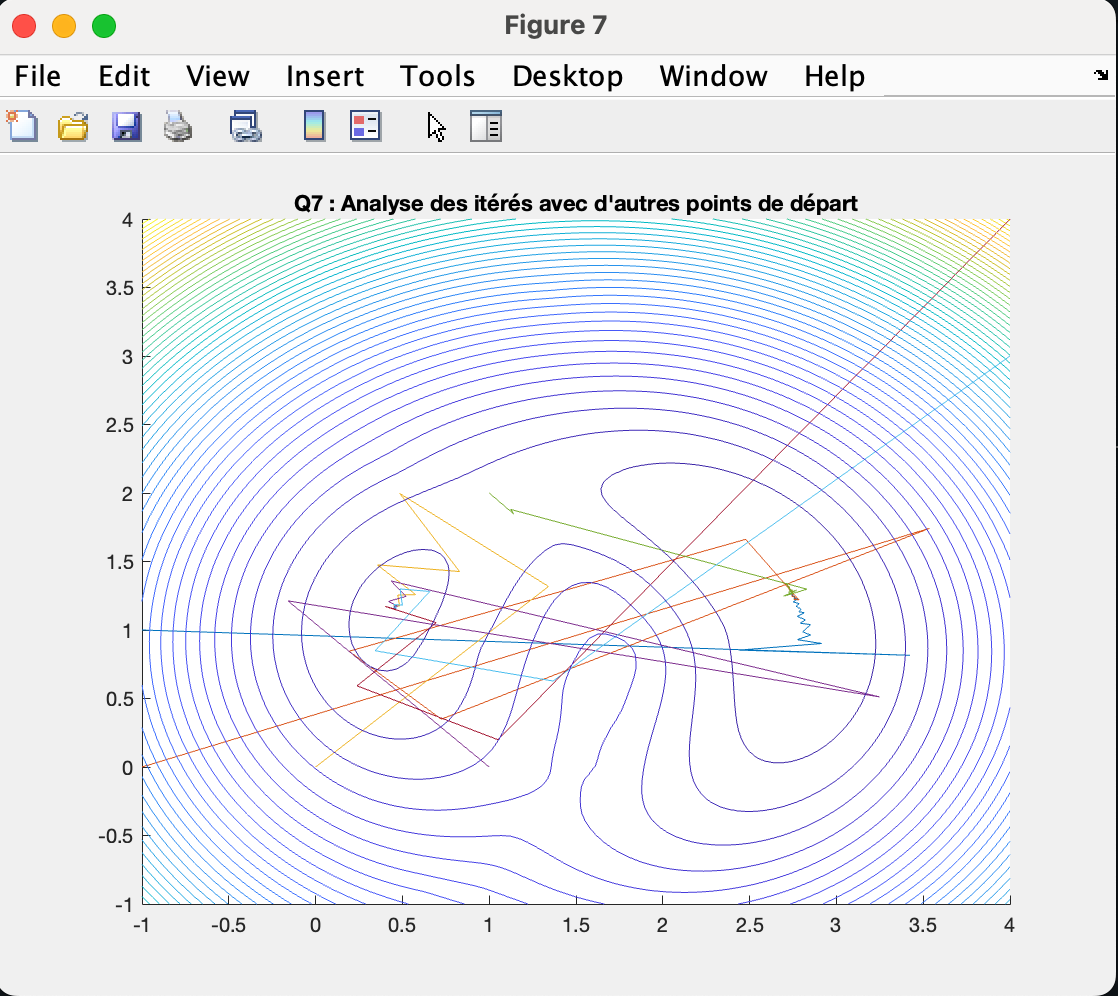
\includegraphics[width=0.8\textwidth]{Q7.png} 
    \caption{Q7 : Répétition de l'étude avec d'autres points de départ}
\end{figure}

\subsection{Question 8}
\begin{figure}[H]
    \centering
    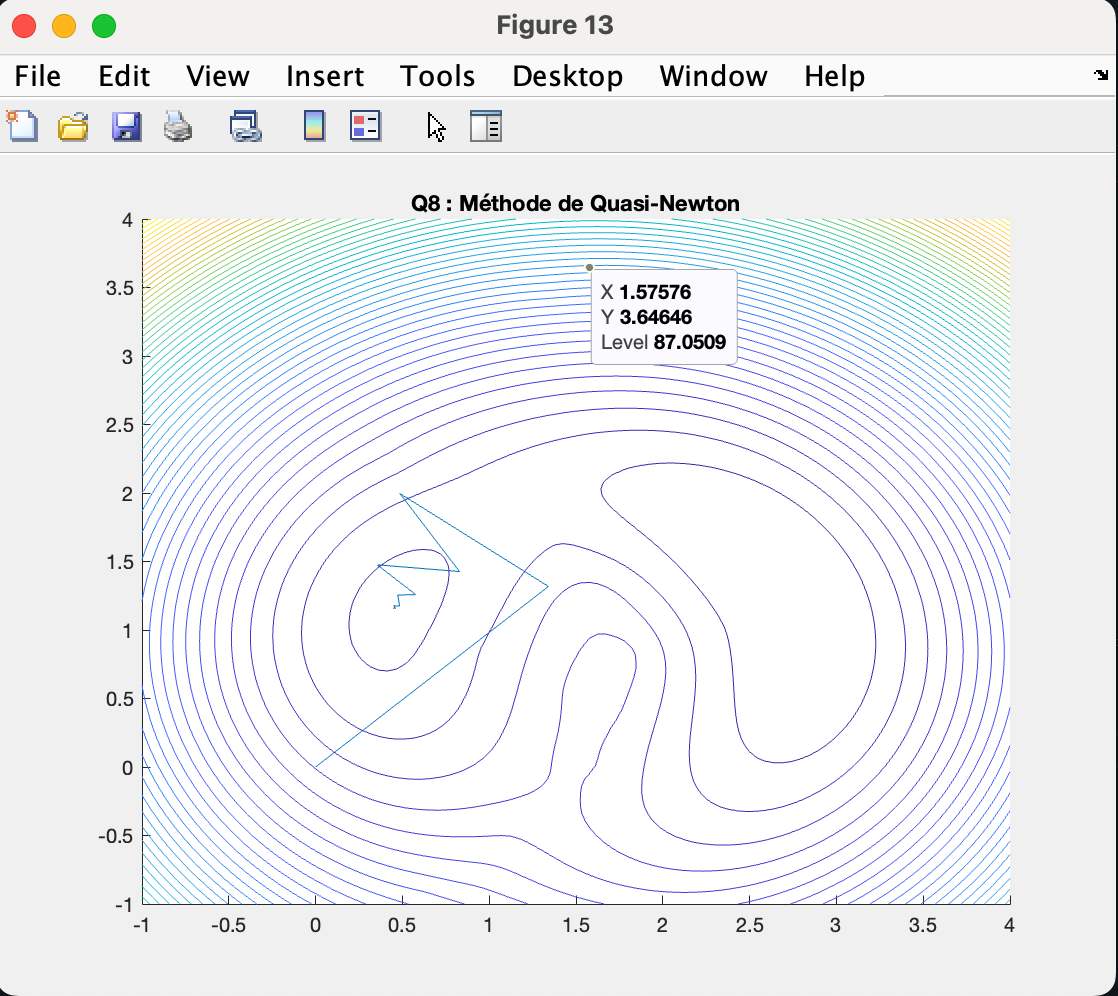
\includegraphics[width=0.8\textwidth]{Q8.1.png} 
    \caption{Q8 : Methode Quasi-Newton}
\end{figure}
\begin{figure}[H]
    \centering
    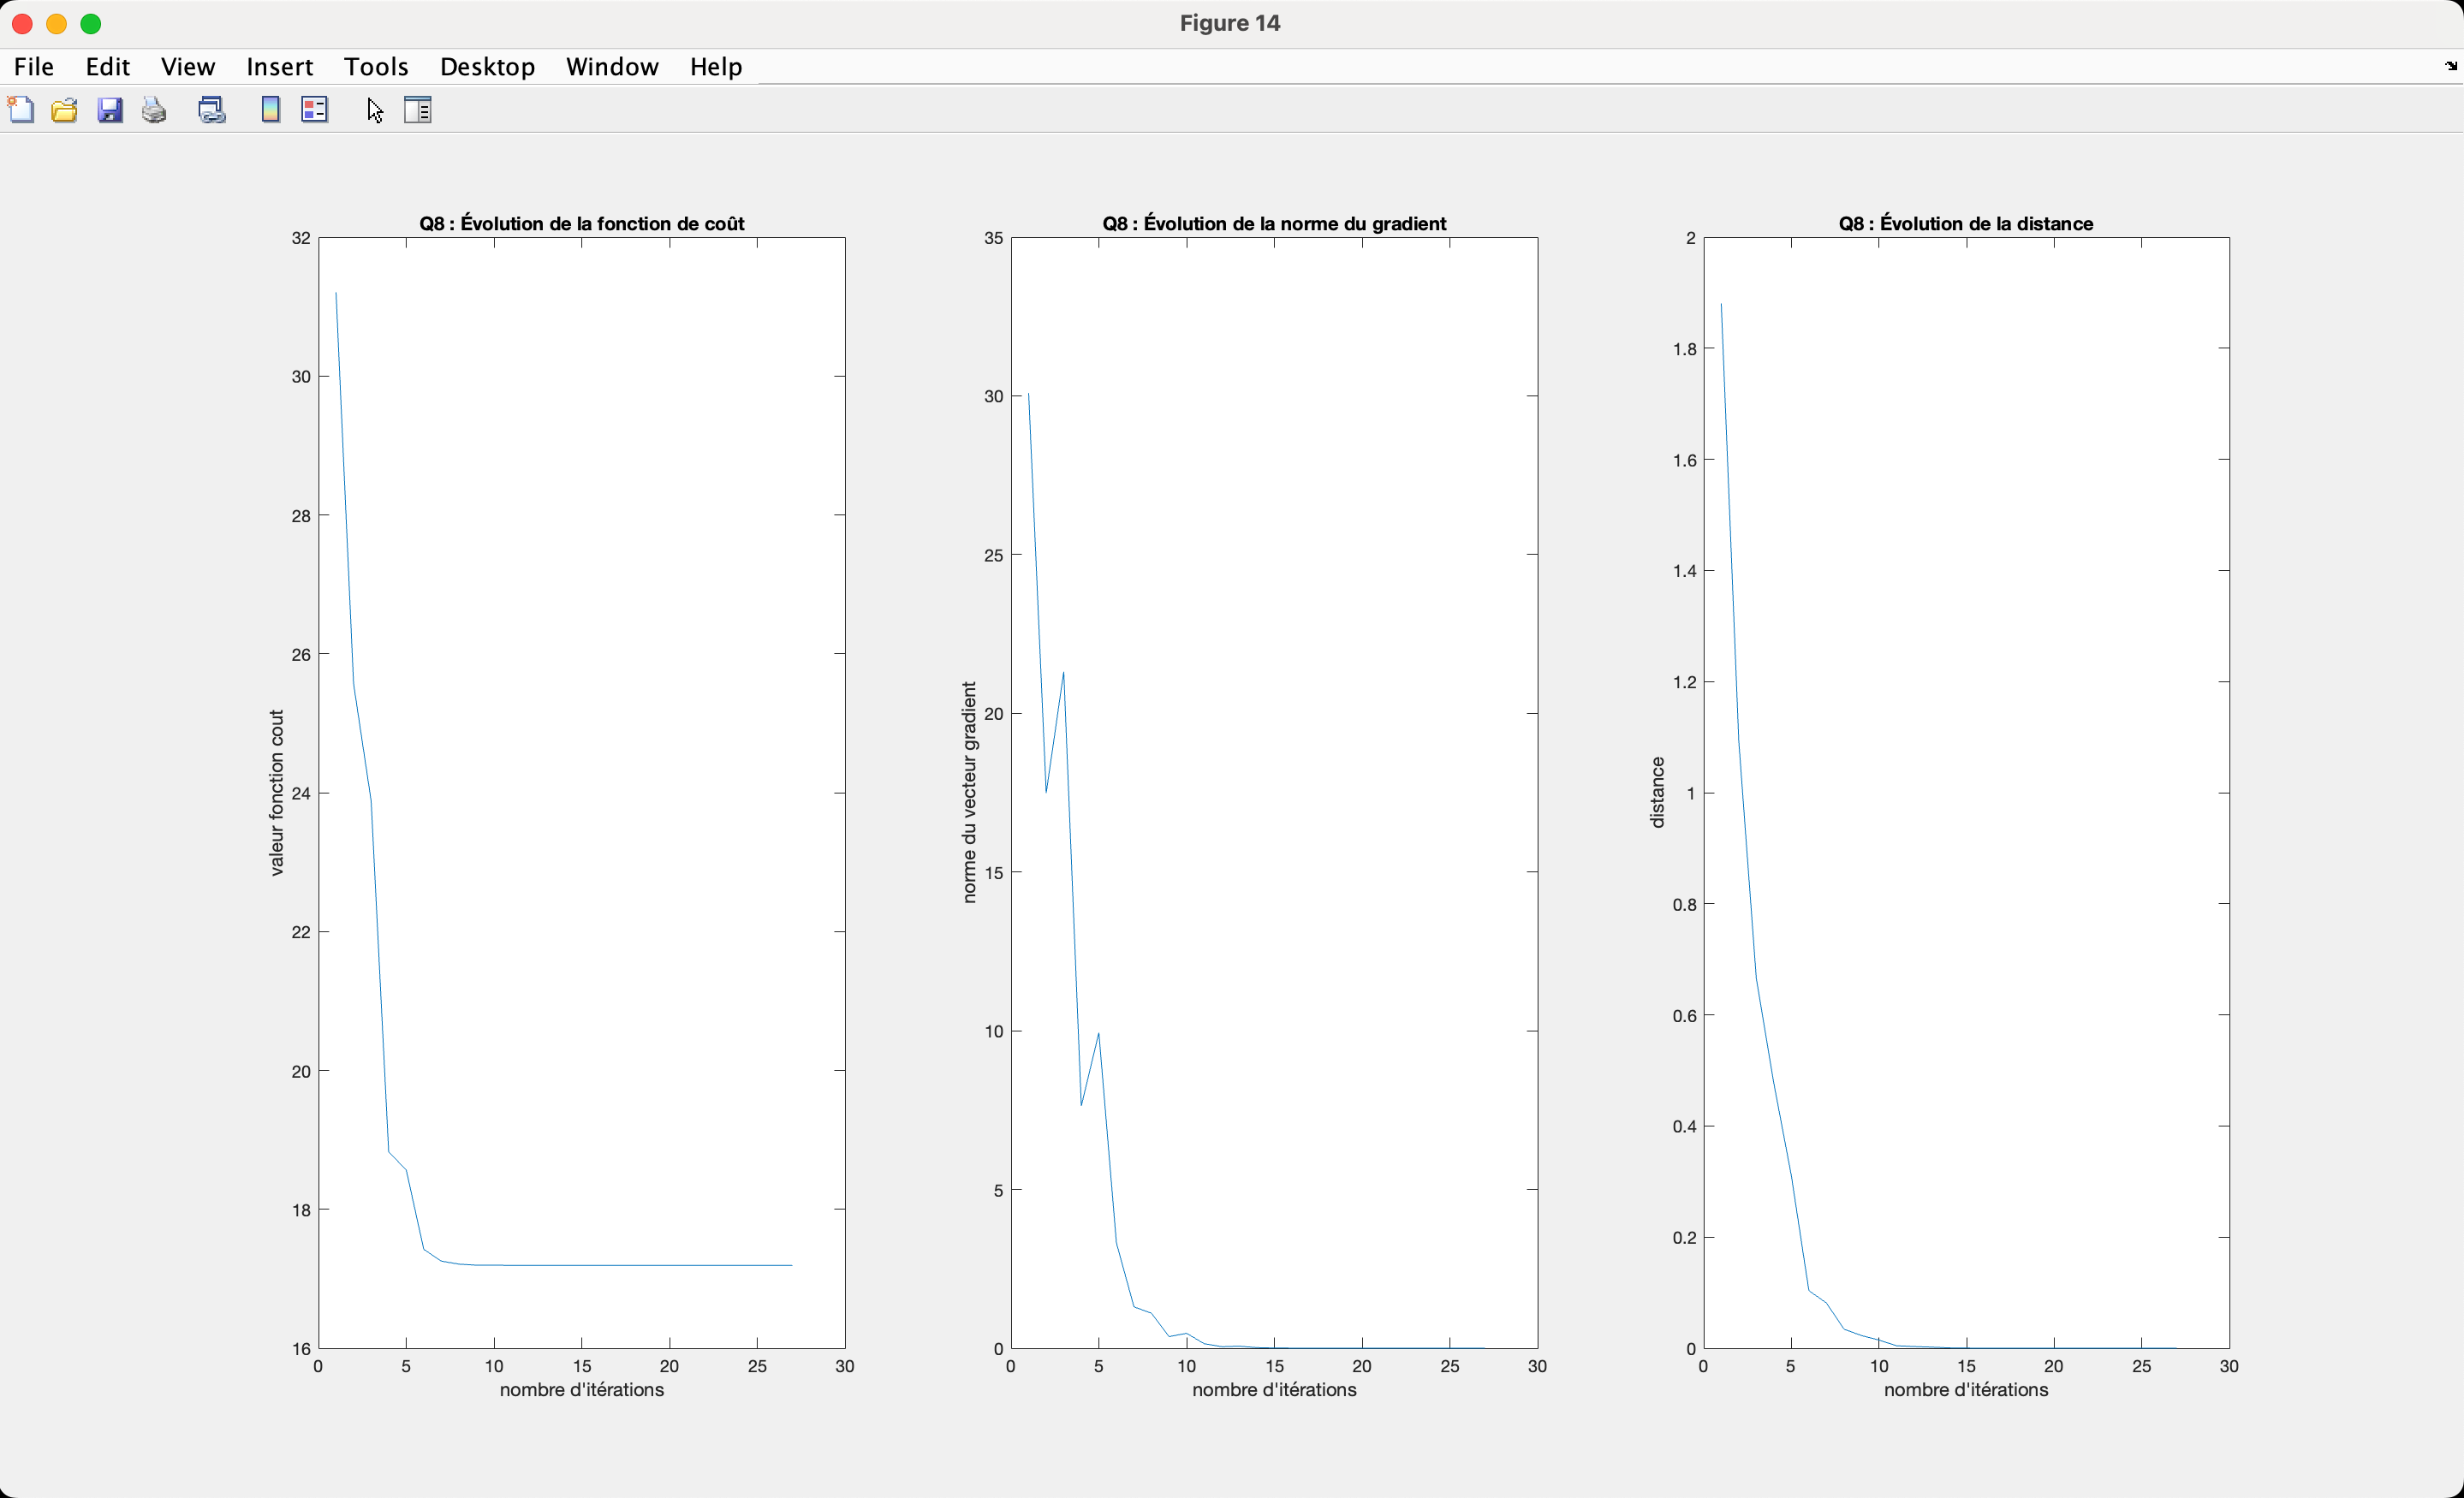
\includegraphics[width=0.8\textwidth]{Q8.2.png} 
    \caption{Q8 : Evolution des différentes caractéristiques demandées}
\end{figure}

\subsection{Question 9}
\begin{figure}
    \centering
    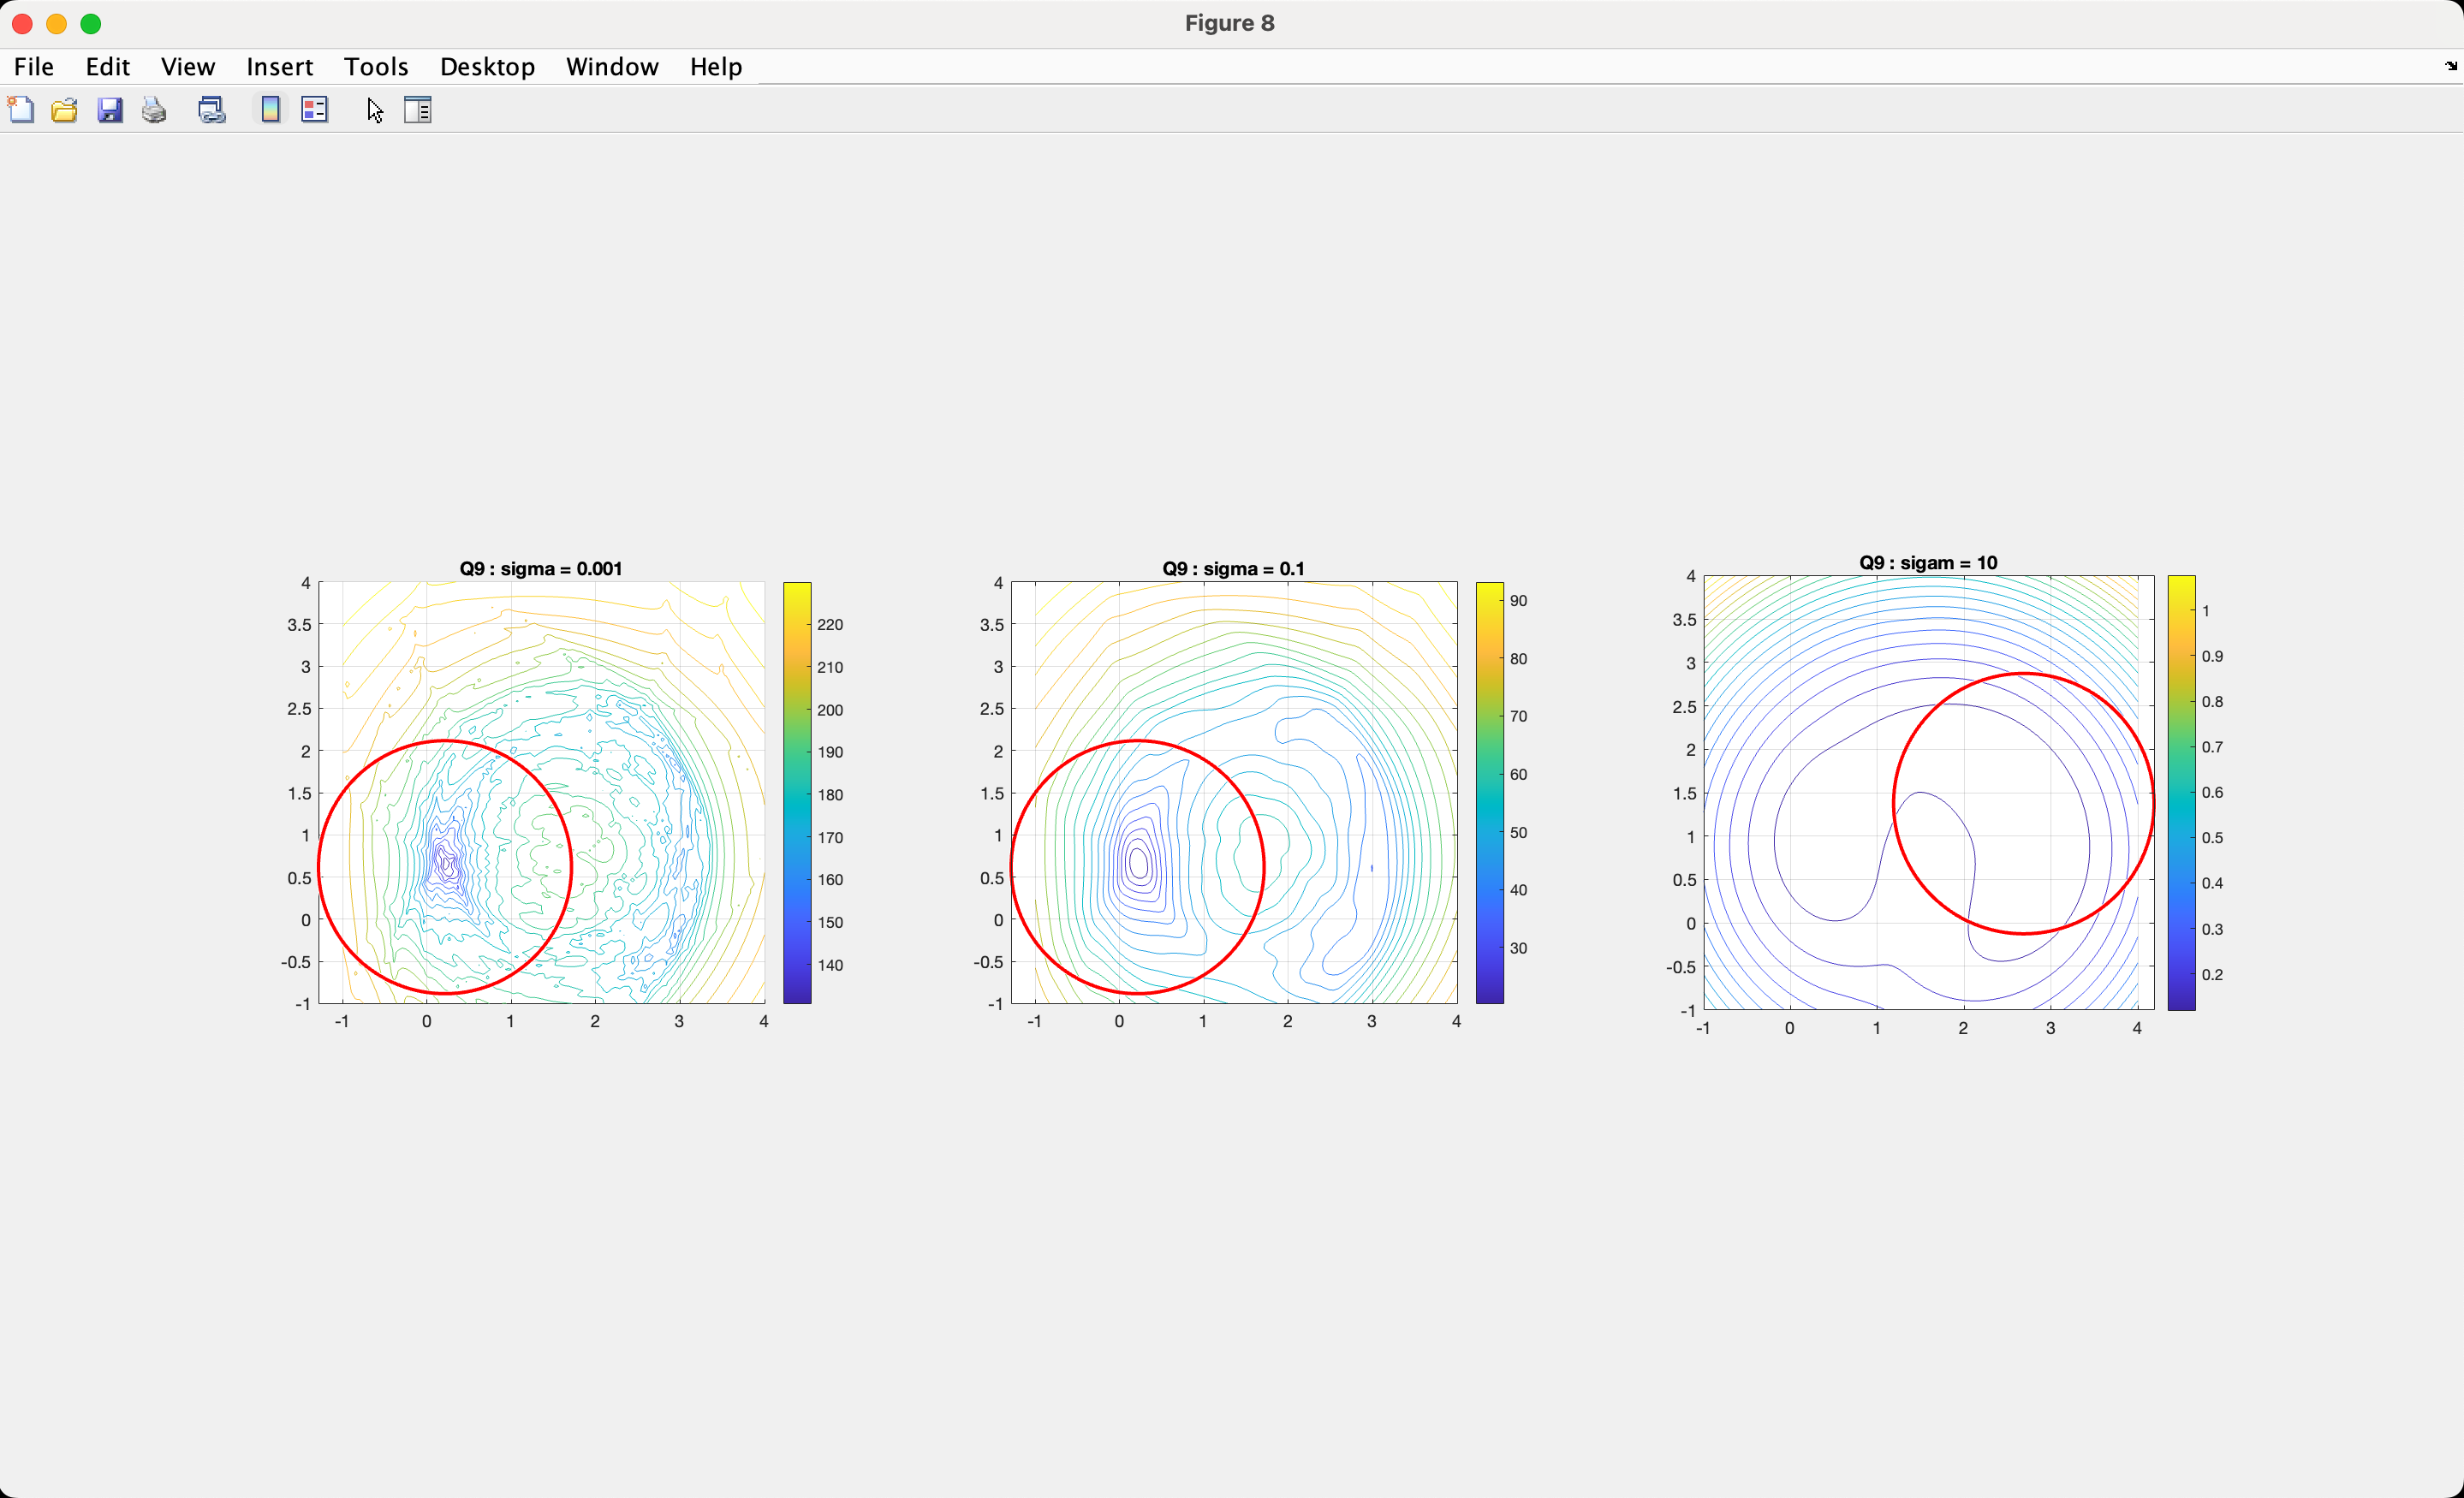
\includegraphics[width=1\textwidth]{Q9.png} 
    \caption{Q9 : Comparaison des différents sigma utilisés}
\end{figure}
La nouvelle fonction de coût nous révèle qu’un choix trop faible de $\sigma$ entraîne une courbe irrégulière, marquée par l’apparition de points aberrants. À l’inverse, si $\sigma$ est trop grand, des informations cruciales sur la courbe sont perdues, et seul un minimum local est alors identifié, au détriment du minimum global. En conséquence, les résultats deviennent exploitables lorsque $\sigma$ se situe dans un intervalle spécifique, avec une valeur intermédiaire de $\sigma$ se révélant être un bon choix.

\subsection{Question 10.3}
Voici la nouvelle expression du gradient de la nouvelle fonction de coût :
\begin{figure}[H]
    \centering
    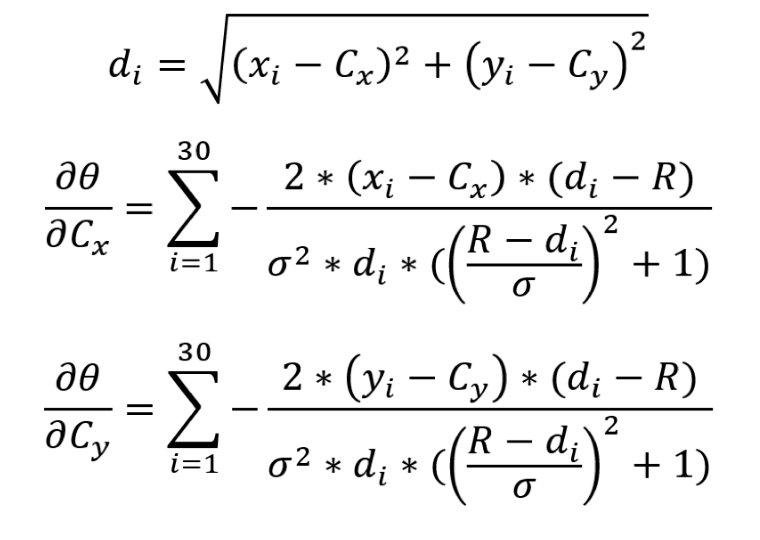
\includegraphics[width=0.5\textwidth]{Q10.3.png} 
    \caption{Expression du gradient de la nouvelle fonction de coût}
\end{figure}

\subsection{Question 10.4}
\begin{figure}[H]
    \centering
    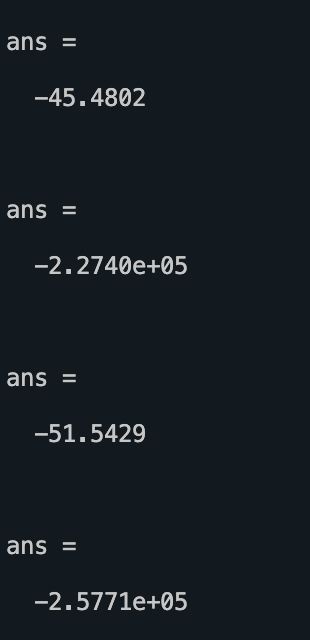
\includegraphics[width=0.3\textwidth]{Q10.4.png} 
    \caption{Q10.4 : Valeurs obtenues pour le point \(0,0\)}
\end{figure}
Les valeurs obtenues pour le point \(0,0\) sont quasiment identiques que la fonction de coût de départ pour certaines valeurs, mais pour d'autres, les valeurs sont complètement erronnées. Ceci suggère une erreur dans le code. 

\subsection{Question 10.5}
\begin{figure}[H]
    \centering
    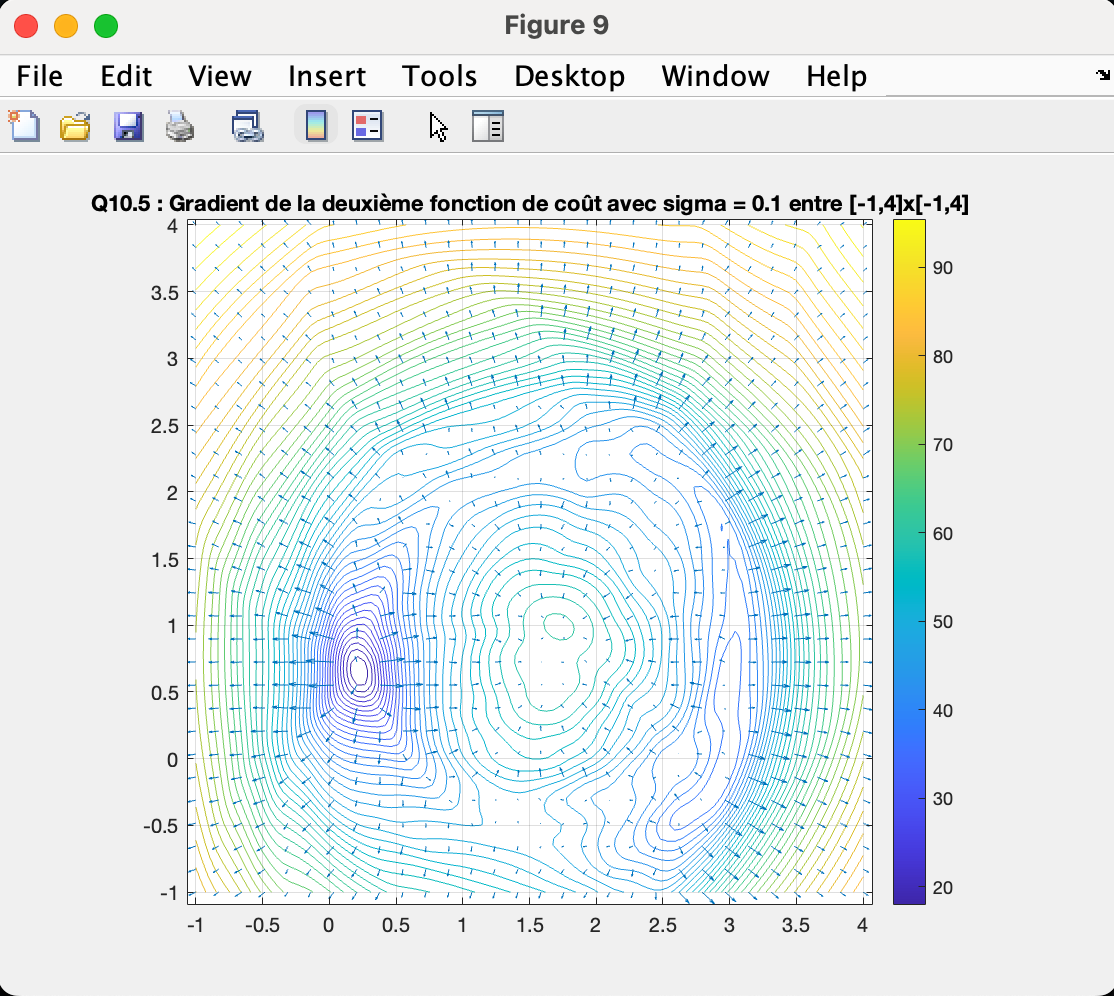
\includegraphics[width=0.8\textwidth]{Q10.5.png} 
    \caption{Q10.5 : Gradient de la nouvelle fonction de coût entre [-1,4]x[-1,4]}
\end{figure}
Il ressort clairement que les vecteurs associés au gradient se trouvent parfaitement perpendiculaires aux courbes de niveau, ce qui atteste de l’exactitude de l’implémentation de la fonction gradient.

\subsection{Question 10.6}
\begin{figure}[H]
    \centering
    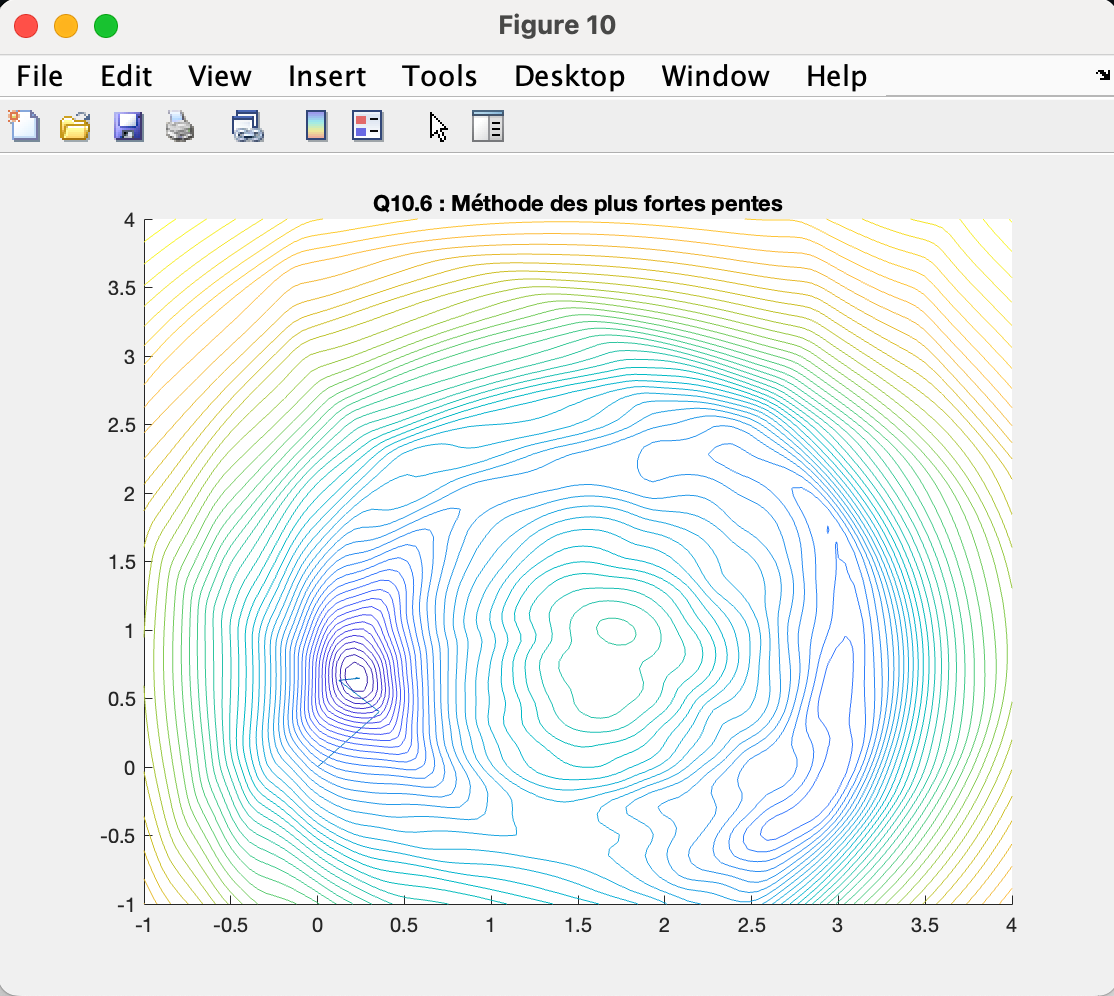
\includegraphics[width=0.8\textwidth]{Q10.6.1.png} 
    \caption{Q10.6.1 : Méthode des plus fortes pentes}
\end{figure}
\begin{figure}[H]
    \centering
    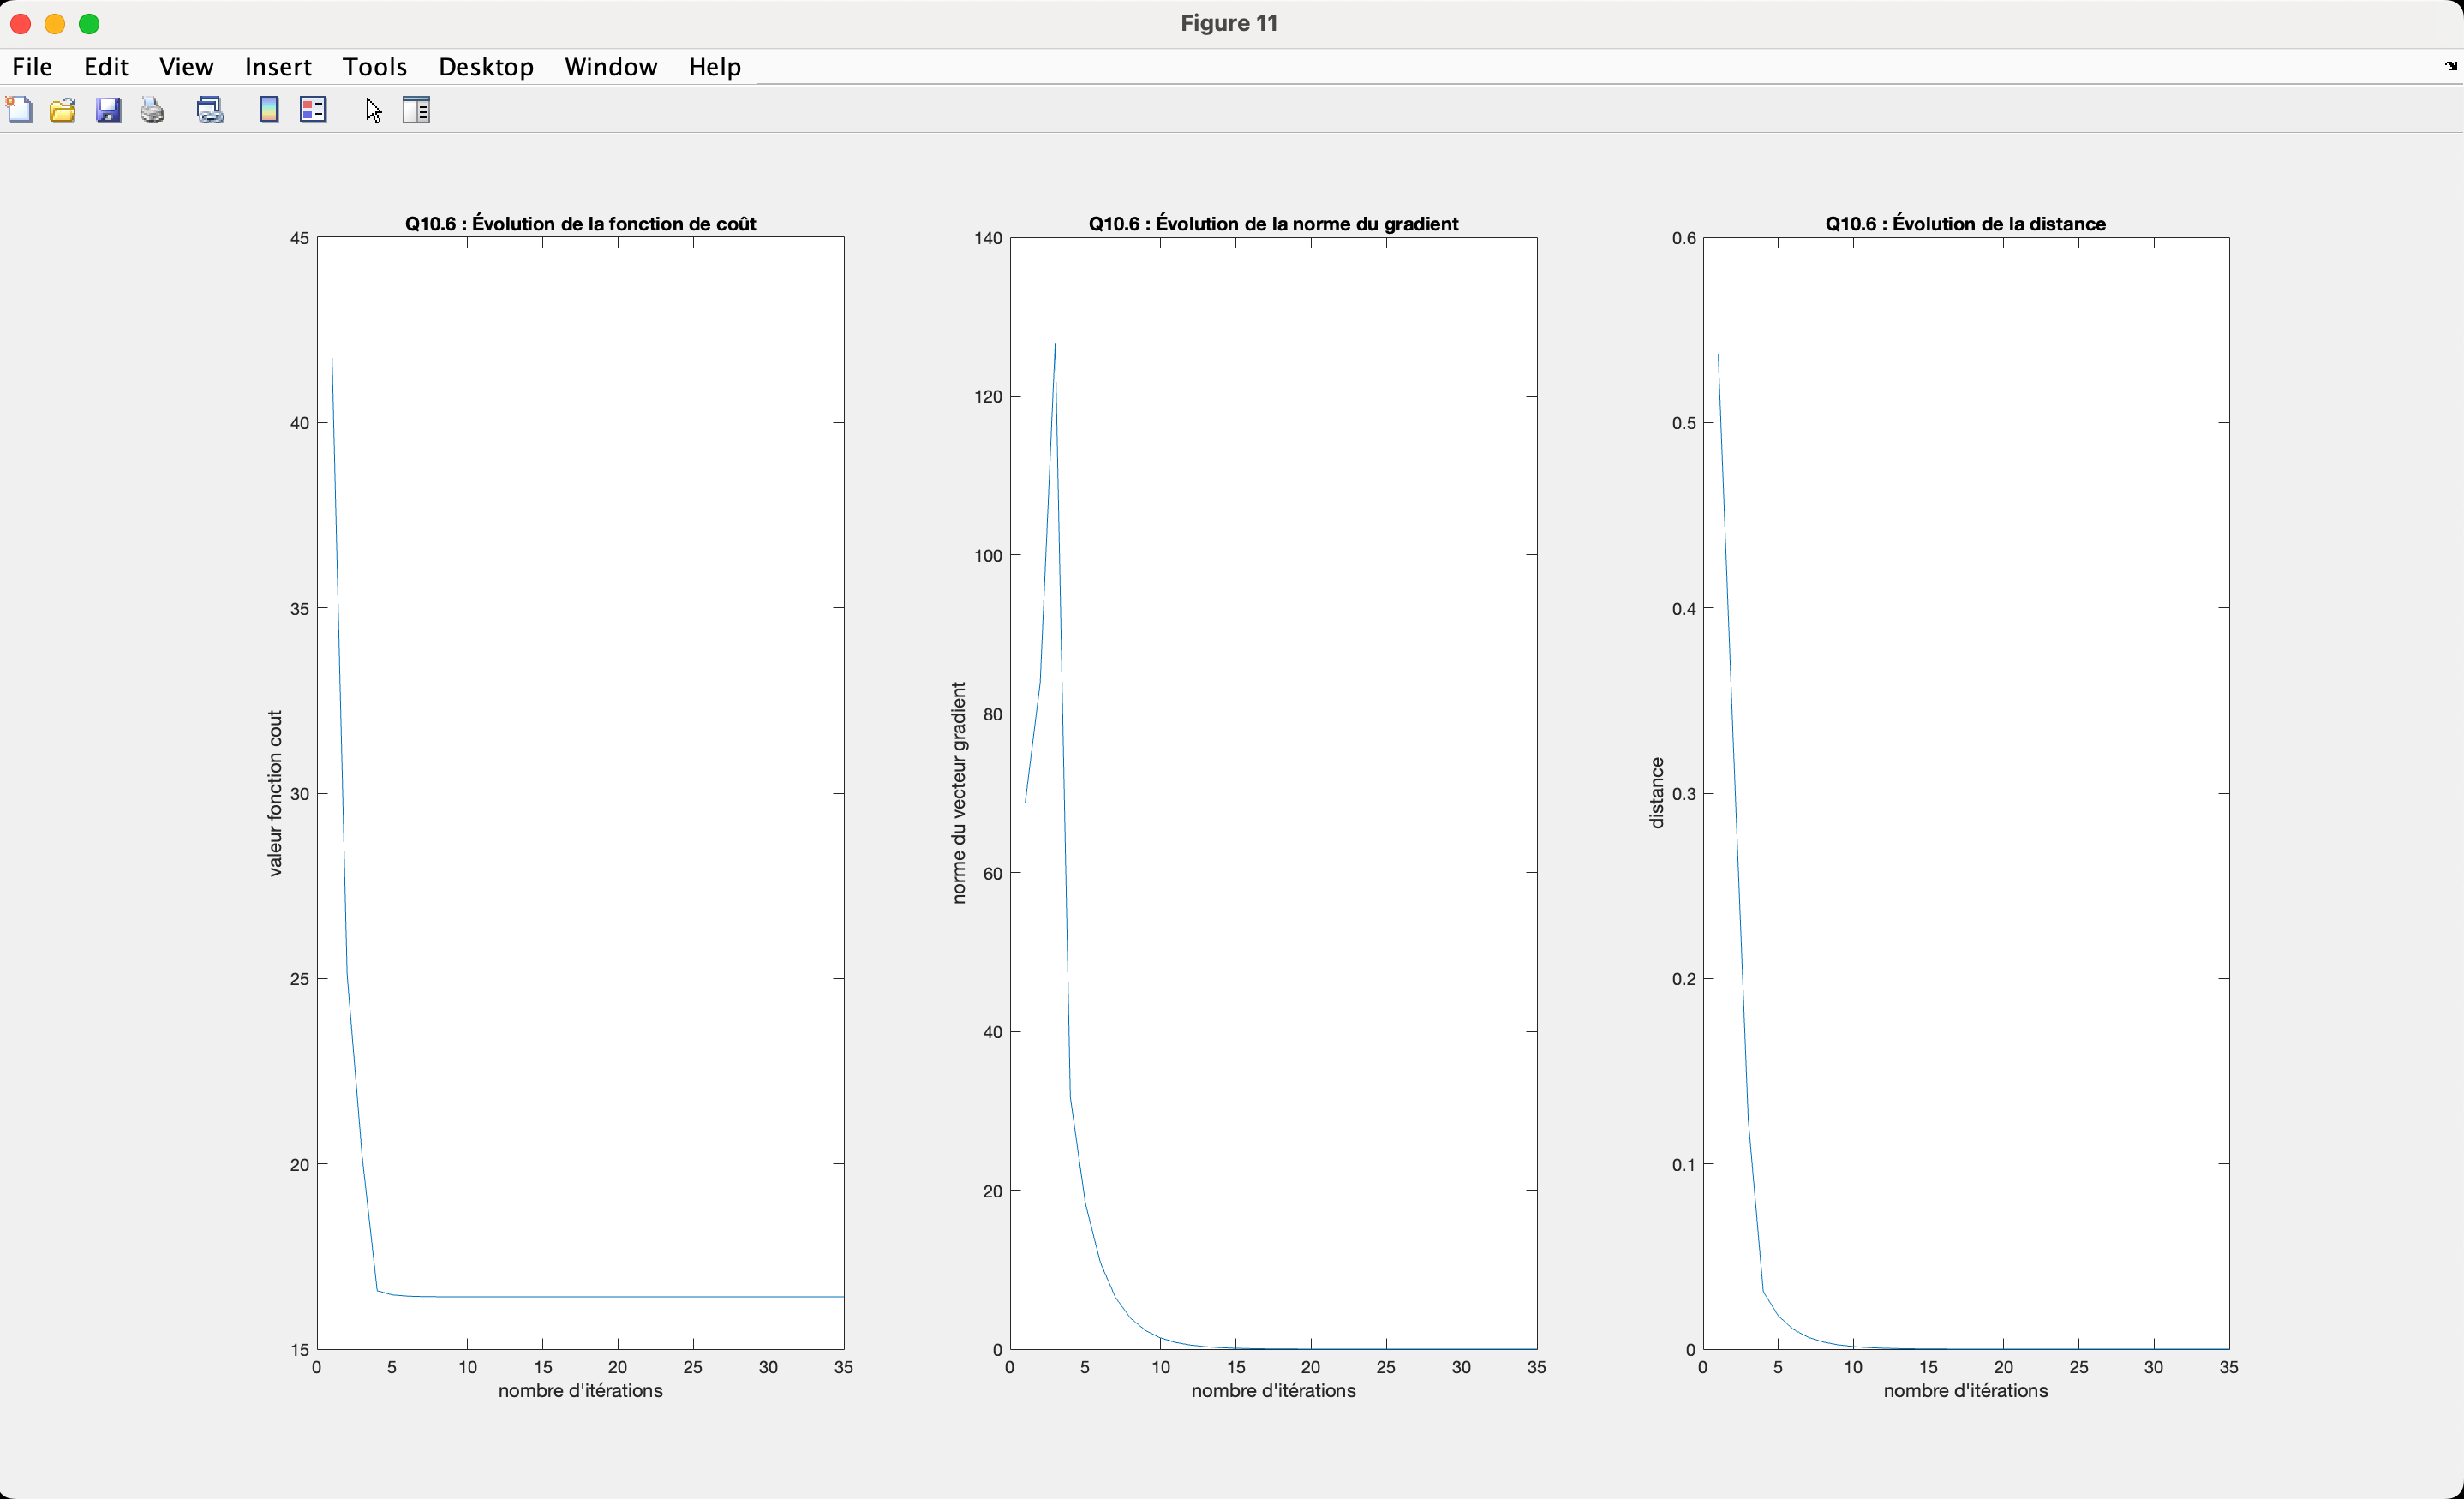
\includegraphics[width=0.8\textwidth]{Q10.6.2.png} 
    \caption{Q10.6.2 : Evolution des différentes caractéristiques demandées}
\end{figure}
Les fluctuations observées dans l’évolution de la fonction de coût, de la norme du gradient et de la distance à la solution suivent des tendances analogues à celles relevées avec l’ancienne fonction de coût. Cependant, la nouvelle formulation se distingue par une convergence plus rapide vers les valeurs finales.

\subsection{Question 10.7}
\begin{figure}[H]
    \centering
    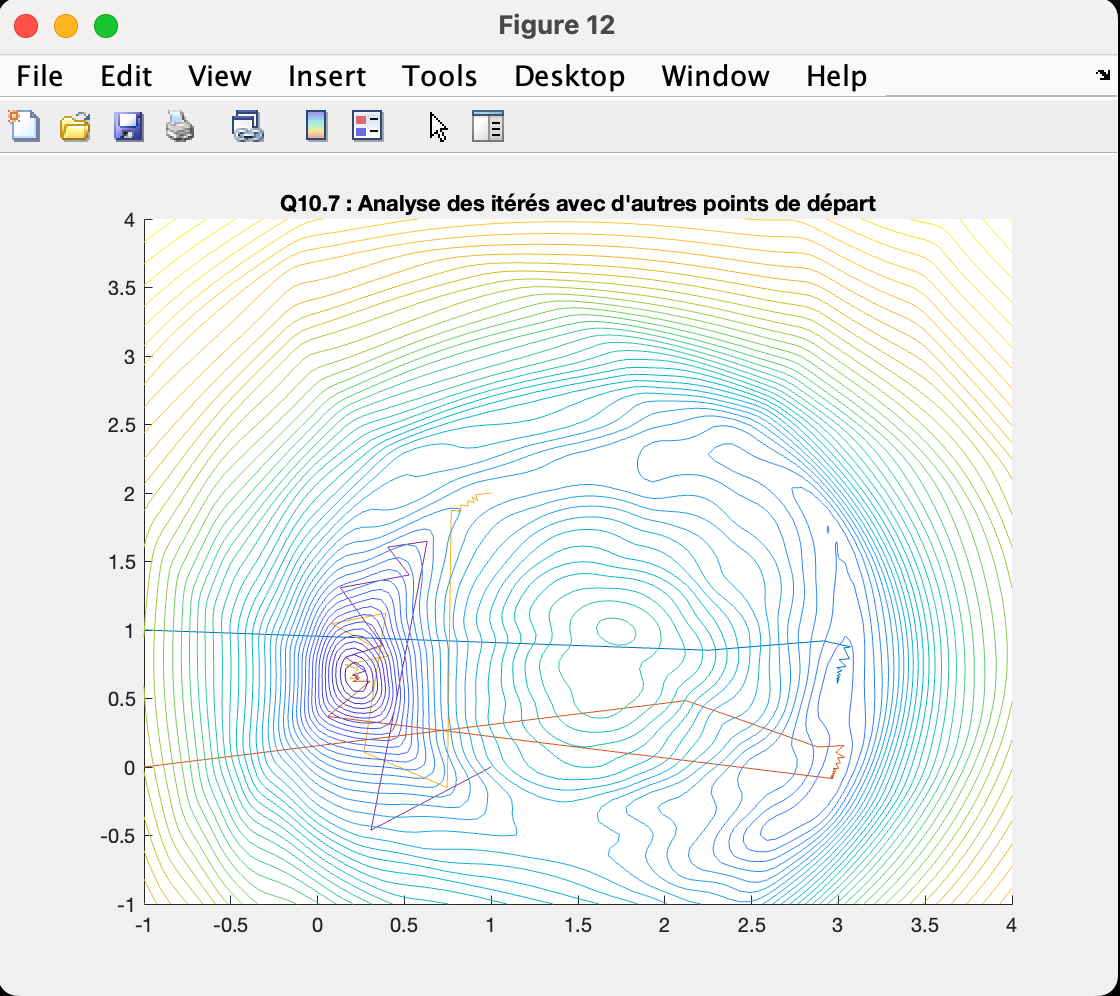
\includegraphics[width=0.8\textwidth]{Q10.7.png} 
    \caption{Q10.7 : Répétition de l'étude avec d'autres points de départ}
\end{figure}
En sélectionnant différents points de départ, il apparaît que la méthode des plus fortes pentes identifie plusieurs minima distincts.
\end{document}